%%
%% Class homework & solution template for latex
%% Alex Ihler
%%
\documentclass[twoside,11pt]{article}
\usepackage{amsmath,amsfonts,amssymb,amsthm}
\usepackage{graphicx,color}
\usepackage{verbatim,url}
\usepackage{listings}
\usepackage{upquote}
\usepackage[T1]{fontenc}
%\usepackage{lmodern}
\usepackage[scaled]{beramono}
%\usepackage{textcomp}

% Directories for other source files and images
\newcommand{\bibtexdir}{../bib}
\newcommand{\figdir}{fig}

\newcommand{\E}{\mathrm{E}}
\newcommand{\Var}{\mathrm{Var}}
\newcommand{\N}{\mathcal{N}}
\newcommand{\matlab}{{\sc Matlab}\ }

\setlength{\textheight}{9in} \setlength{\textwidth}{6.5in}
\setlength{\oddsidemargin}{-.25in}  % Centers text.
\setlength{\evensidemargin}{-.25in} %
\setlength{\topmargin}{0in} %
\setlength{\headheight}{0in} %
\setlength{\headsep}{0in} %

\renewcommand{\labelenumi}{(\alph{enumi})}
\renewcommand{\labelenumii}{(\arabic{enumii})}

\theoremstyle{definition}
\newtheorem{MatEx}{M{\scriptsize{ATLAB}} Usage Example}

\definecolor{comments}{rgb}{0,.5,0}
\definecolor{backgnd}{rgb}{.95,.95,.95}
\definecolor{string}{rgb}{.2,.2,.2}
\lstset{language=Matlab}
\lstset{basicstyle=\small\ttfamily,
        mathescape=true,
        emptylines=1, showlines=true,
        backgroundcolor=\color{backgnd},
        commentstyle=\color{comments}\ttfamily, %\rmfamily,
        stringstyle=\color{string}\ttfamily,
        keywordstyle=\ttfamily, %\normalfont,
        showstringspaces=false}
\newcommand{\matp}{\mathbf{\gg}}

\begin{document}

\section*{Introduction: Decision Tree Methods}

In order to fully test decision trees and see if that method works best for the data, we tested multiple decision tree methods. This meant comparing a single strong decision tree with multiple weak decision trees. With the weak decisiont trees, we also compared ways of boosting and ensembling them. I also added two features: the mean and standard deviation of the IR3 image patch (the X2 data set). Adding this data could only help since decision trees could leave out the features if they don't matter. 

\section*{Single Decision Tree} 

In order to optimize a single decision tree, I tested the hyperparameters of minParent and maxDepth. With minParent, it was clear that the ideal value for our data set was $2^9$ from the work we did in Homework 4. The validation error curve clearly showed that $2^9$ was the best value and it began to overfit after that. With maxDepth, the ideal value seemed to have been 15 but I wanted to see if a larger maxDepth would be better or cause the data to overfit. 
\begin{figure}[h]
\centering
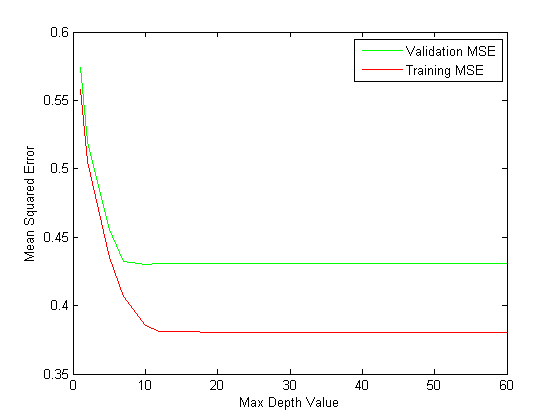
\includegraphics[width=4 in]{maxDepthVersusMSE.png}
\caption{MaxDepth Versus MSE}
\end{figure}

\newpage 

As can be observed, once the maxDepth value reaches 20 or so, the training and validation error stays relatively the same. Since the minParent value was $512$, it is likely that after 20 layers, the decision tree does not have enough data in each node for meaningful splits. In order to verify this, I lowered the minParent value to $32$ to see if we will have the same effect as above, but after a greater number of layers. As it turns out, at 30 layers, the training error stops improving. When you look at the validation error though as a function of maxDepth, it is clear that there is overfitting after about 7 layers. Hence having a low minParent value not only causes more layers to occur but also increases overfitting.  \\
\begin{figure}[h]
\centering
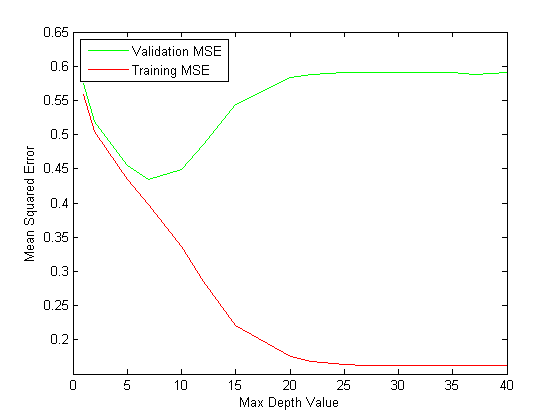
\includegraphics[width=4 in]{maxDepthVersusMSE2.png}
\caption{MaxDepth Versus MSE}
\end{figure}

In the end, the best validation error occcured with minParent equal to 512 and the maxDepth equal to 20, so that is what I used when making the Kaggle data set. The Kaggle MSE ended up being 0.65003. 

\newpage

\section*{Gradient Boosting}

For Gradient Boosting, the goal is to combine together weak decision trees by boosting each one based on the residual errors from the previous tree. In order to reduce the complexity of an individual tree, I set the maxDepth to 3 and the minParent to 512. I wanted to see how increasing the number of boosted learners affects the training and validation MSE. As it turns out, after about 50 learners, the training error does decrease but the validation error stays relatively constant. This suggests that even though it has started fitting to the data at that point, it is not very dramatic overfitting. After retraining on all the training data, using 150 boosted learners, and submitting the results to Kaggle, the MSE was 0.61388. \\
\begin{figure}[h!]
\centering
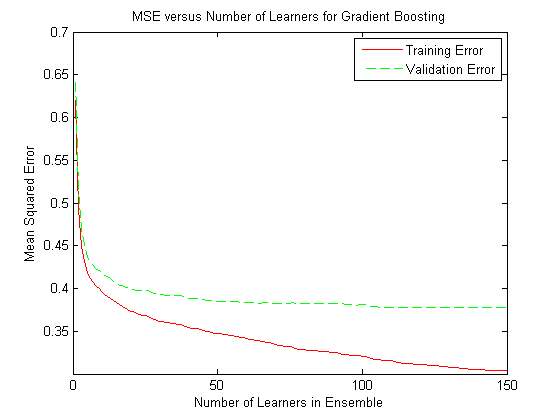
\includegraphics[width=4 in]{numGradBoostsVersusMSE.png}
\caption{Gradient Boosting Versus MSE}
\end{figure}

\newpage

\section*{Random Forests}

For random forests, we tried making each learner weak in that it only looks at a subset of the features. We then average together the results of each learner in an effort to boost performance. The hyperparameters we cared about were the number of learners used as well as the number of features selected randomly. I decided to first test the number of features and see if there was a clear ideal value. I had it learn 10 learners in each case. If there were more learners, then the performance difference might not be so dramatic. Initially, there was a big difference in validation MSE but after 40 or more features, adding more did not improve it much. This is likely because only around 40 of those features matter in predicting the outcome and the other features are extra. I decided to stick with 40 features for my test of the number of learners. \\

\begin{figure}[h!]
\centering
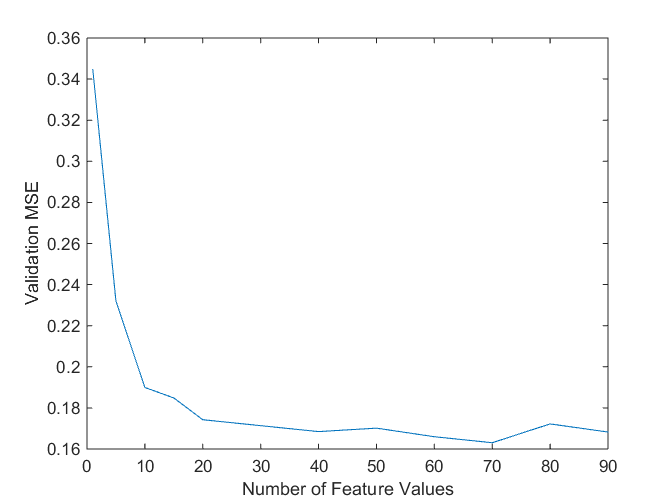
\includegraphics[width=4 in]{numFeatValuesVersusMSE.png}
\caption{Number of Random Features versus Validation MSE}
\end{figure}

\newpage

Next I tested how many learners it takes to get a good validation MSE. As it turns out after about 60 learners, the model stops improving. The following graph shows this. Because we bootstrap the data, the training MSE shown is actually the training MSE for each individual learner. \\

\begin{figure}[h!]
\centering
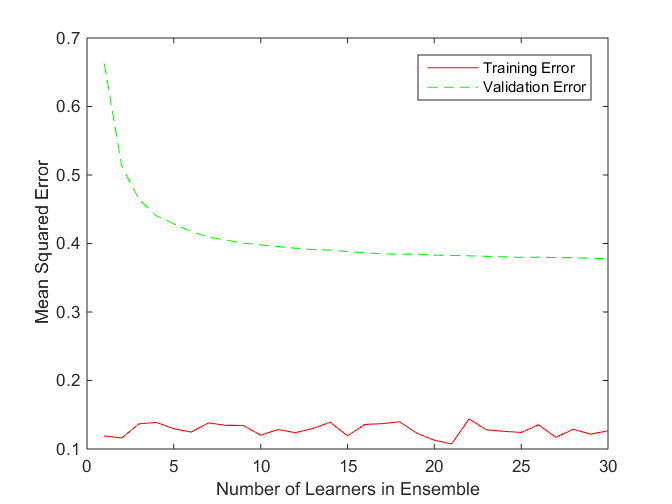
\includegraphics[width=4 in]{numLearnersVersusMSE.png}
\caption{Number of Learners versus MSE}
\end{figure}

After these tests, I ran random forests with 40 features and on 60 weak learners. The Kaggle MSE ended up being 0.60282. 

\newpage

\section*{Gradient Boosted Random Forests}

Seeing the sawtooth pattern with the training error caused me to hypothesize that some of those sets of features are likely better than others. I thus decided to see if gradient boosting these particular learners and then ensembling the results would achieve good results. \\
\\
I did the following procedure:\\
1. Train decision trees on random sets of 40 features\\
2. Take the 30 best sets of features and train boosted decision trees on them\\
3. Ensemble the trees from step 2\\
\\
After training 50 different random learners with a different random feature set for each, this is the graph of training and validation MSE that I observed.
\begin{figure}[h!]
\centering
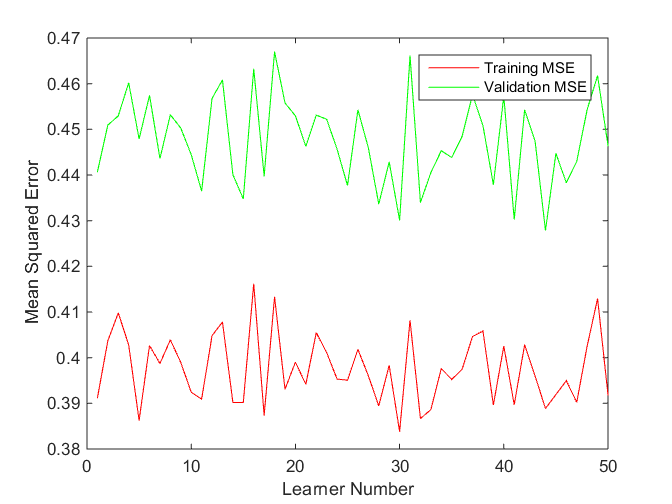
\includegraphics[width=4 in]{learnerNumVersusMSE.png}
\caption{Learner Number versus MSE}
\end{figure}

I then took the best feature sets in order and gradient boosted their decision trees. I ensembled the trees and here is the validation and training MSE that resulted:

\begin{figure}[h!]
\centering
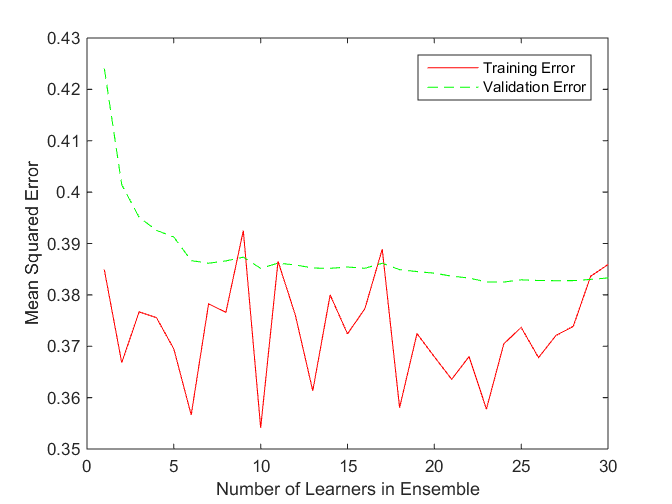
\includegraphics[width=4 in]{numLearnersVersusMSE2.png}
\caption{Number of Learners versus MSE}
\end{figure}

Unfortunately, the results were not too impressive and did not beat normal random forests. After uploading to Kaggle, the MSE was 0.61502. 

\newpage

\section*{Conclusion}

After trying different decision tree methods, it turns out that normal random forests beat all the other methods. The number of features to make random forests optimal was still quite high. This suggests that there is a relationship among the input features that makes direct decision trees a great method for approximating the output. However, which exact features they are is difficult to say hence it's best when you ensemble a few different guesses of which features are good. 

\end{document}
